		\documentclass{scrartcl}
		\usepackage{amsmath,graphicx,booktabs,amssymb,tikz,accents,mathtools,empheq,multicol}
		\usetikzlibrary{positioning}
		\usepackage[margin=.7in]{geometry}
		\newcommand{\rb}[1]{\ensuremath{\left(#1\right)}}
		\newcommand{\sqb}[1]{\ensuremath{\left[#1\right]}}
		\newcommand{\sgb}[1]{\ensuremath{\left\{#1\right\}}}
		\newcommand{\vb}[1]{\ensuremath{\left\langle#1\right\rangle}}
		\newcommand*\diff{\mathop{}\!\mathrm{d}}
		\newcommand{\ubar}[1]{\underaccent{\bar}{#1}}
		\def\exp{\mathbb{E}}
		\def\uni{\cup}
		\def\chil{\ensuremath{\rho}}

		\begin{document}

			\begin{center}
				\huge
				\underline{``Market Fragmentation \& Speed'' Proposal v8} \\
				\LARGE
				Soomin ``Tomy'' Lee - \today
			\end{center}

			\subsection*{Research Question}
			\begin{itemize}\itemsep.1em
				\item Can high frequency liquidity providers enhance price discovery?
			\end{itemize}

			\subsection*{Motivation}
			\begin{itemize}\itemsep.1em
				\item HF market makers (HFMMs) improve price efficiency/discovery
				\begin{itemize}
					\item Reduce returns (Skjeltorp et al [2013 WP]), reduce prices to random walk (Conrad et al [2015 JFE]), reduce volatility (Hagstromer and Norden [2013 JFM])
				\end{itemize}
				\item New exchanges explicitly discouraging HFT activity (low latency exchanges)
				\begin{itemize}
					\item e.g. Aequitas (Canada), IEX (US)
				\end{itemize}
			\end{itemize}

			\subsection*{Intuition}
			\begin{itemize}\itemsep.1em
				\item HFMMs rapidly extract information across markets and revise quotes
				\item HFMMs facilitate competition among ITs in different markets
				\item Above competition enhances price discovery
				\item[$\implies$] Low latency markets may attract some ITs
				\item[$\implies$] Those ITs face reduced competition (since MMs cannot view other orderflows)
				\item[$\implies$] Such ITs trade less aggressively and impose externalities on HF markets
			\end{itemize}

			\subsection*{Market aspects modelled}
			\begin{itemize}\itemsep.1em
				\item Fragmented markets (markets with often separate investors trading the same asset)
				\item Ability to monitor across markets (``speed'')
				\item Heterogenous markets (HF or low frequency)
			\end{itemize}

			\subsection*{Similar Papers}
			\begin{itemize}\itemsep.1em
				\item Foucault, Kozhan and Tham (2015 WP) ``Toxic Arbitrage'' [fast arbitragers/slow MMs]
				\item Biais, Foucault and Moinas (2015 JFE) ``Equilibrium Fast Trading'' [fragmented markets]
				\item Back, Cao and Willard (2000 JF) ``Imperfect Competition among Informed Traders''
				\item Pasquariello and Vega (2007 RFS) ``Informed and Strategic Order Flow in the Bond Markets'' [heterogenous signals]
			\end{itemize}

			\subsection*{Contribution}
			\begin{itemize}\itemsep.1em
				\item Unlike FKT or BFM, focus on liquidity providers/MMs being fast
				\item Unlike BCW or PV, examine \emph{disaggregated} informed orderflows
				\item Examine a potential channel for HFTs' market-improving effects
			\end{itemize}

			\subsection*{Elements of the General Model}
			\begin{itemize}\itemsep.1em
				\item Based on Kyle (1985)
				\item $M$ markets trading same asset with value $v$
				\item Each market contains an informed trader, competitive MM and noise traders
				\item ``MM'' represents all uninformed but rational traders who maximize returns
				\item ITs receive stochastic signal $s_i$ at start of time 0
				\item MM in market $i$ observe $y_{it} = x_{it} + u_{it} $ and $y_{jt}, \, \forall j$ 
			\end{itemize}

			\subsection*{Extentions}
			\begin{enumerate}
				\item $N < M$ markets are low frequency 
				\begin{itemize}
					\item MMs cannot observe $\{y_{js}\}_{j\neq i} $ for $s \in (t-\varepsilon,t], \, \varepsilon \in (0,1) $ %)
				\end{itemize}
				\item $v$ evolves according to a stochastic process% and a signal is sent to ITs each period
			\end{enumerate}

			\subsection*{Plan}
			\begin{enumerate}
				\item Solve a baseline model where MMs cannot observe other markets' orderflows
				\item Solve the general model where each MM can observe every markets' orderflows
				\item Solve the model where $N$ markets are low frequency
				\item Compare price efficiency among the above cases  
			\end{enumerate}

			\subsection*{Model Setup}
			\begin{description}
				\item[Asset] Single asset with value $v \sim N(\mu,\sigma_v^2) $ traded across $M > 1$ markets
				\item[Time] Continuous trading between $t = [0,1)$
				\item[Agents] Each market $i$ consists of an informed trader (IT), a market maker (MM), and noise traders
				\item[Actions] $t$ subscripts below denote period-$t$ and market index $i$ are omitted:
				\begin{enumerate}
					\item[\textbf{IT}] \makebox[1.5cm][l]{$X(IT) $} $= \mathbb{R} $, $x_t \in X $ denotes IT's orderflow
					\item[\textbf{MM}] \makebox[1.5cm][l]{$P(MM) $} $= \mathbb{R}_{++} $, $p_t \in P $ denotes price
					\item[\textbf{NT}] \makebox[1.5cm][l]{$Z(NT) $} $= \mathbb{R},\, z_t \sim N(0,\sigma^2_n) $ denotes noise traders' net orderflow
					\item[Note] $y_t = x_t + z_t$ denotes the total orderflow
				\end{enumerate}
				\item[Information] Below holds for all $j\in\{1,\ldots,M\} $:
				\begin{enumerate} 
					\item[\textbf{IT}] Gets signal $s_i $ where $ [s_1,\ldots,s_M]' \sim N(\mathbf{0},\Sigma) $. The $M$-by-$M$ matrix $\Sigma$ has diagonal elements $\{\sigma_a^2\}_{a=1}^M $ and off diagonal elements $\{\sigma_{ab}\} $ in $a$th row $b$th column, $a \neq b$.
					\item[] Normalize s.t. $v = \mu + \sum_{j=1}^M s_j $\footnote{As in Foster and Viswanathan (1996 JF) and BCW}
					\item[] \makebox[.6cm][l]{$\mathcal{I}_{it} $} $= \{s_i\}\uni\{p_{j,q}\,,\,y_{j,q}\}_{q<t} $
					\item[\textbf{MM}] \makebox[.6cm][l]{$\mathcal{M}_{it} $} $= \{p_{j,q}\,,\,y_{j,q}\}_{q<t} \uni \{y_{j,t}\} $
					\item[\textbf{NT}] \makebox[.6cm][l]{$\mathcal{N}_{it} $} $= \varnothing $
				\end{enumerate}
				\item[Payoffs] At the end of time $t$\dots
				\begin{enumerate}
					\item[\textbf{IT}] \makebox[1.7cm][l]{$\Pi_{it}(IT) $} $ = \int_0^t x_{i,q}(v - p_{i,q})\diff q $
					\item[\textbf{MM}] \makebox[1.7cm][l]{$\Pi_{it}(MM) $} $ = \int_0^t y_{i,q}(p_{i,q} - v)\diff q $
				\end{enumerate}
				\item[Timing] For markets $i\neq j$:\\
			\end{description}
			\vspace{-1em}
			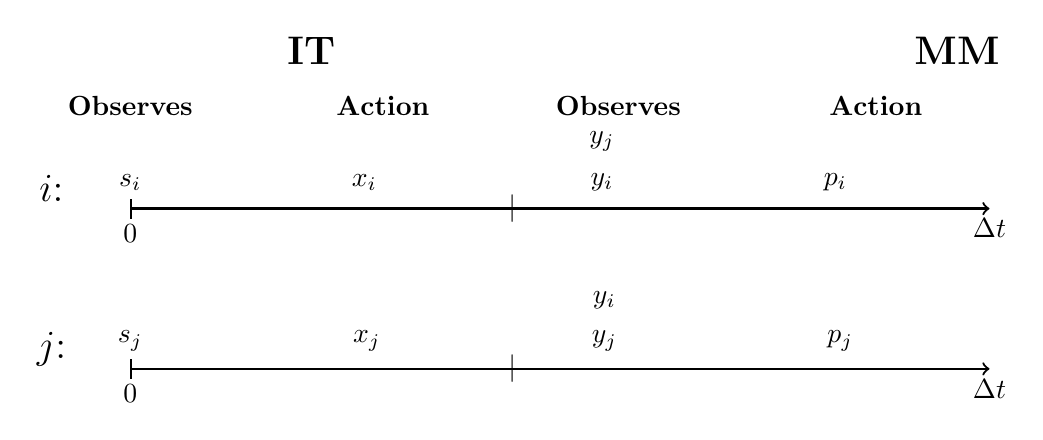
\begin{tikzpicture}
				\coordinate (a) at (0,0);
				\node [above = 2em of a] (b) {\Large $i$:};              \node [below = 2em of a] (c) {\Large $j$:};
				\draw [|->,thick] (b) ++(1,-.25) node[below=2pt] (d) {0} -- +(.4\textwidth,0) node {$|$} -- ++(.9\textwidth,0) node [anchor=north] {$\Delta t$};
				\draw [|->,thick] (c) ++(1,-.25) node[below=2pt] (e) {0} -- +(.4\textwidth,0) node {$|$} -- ++(.9\textwidth,0) node [anchor=north] {$\Delta t$};
				\node [above = .5em of d] (f) {$s_i$};                   \node [above = .5em of e] (g) {$s_j$};
 				\node [right = .2\textwidth of f] {$x_i$};               \node [right = .45\textwidth of f] (h) {$y_i$};
				\node [right = .2\textwidth of g] {$x_j$};               \node [right = .45\textwidth of g] (i) {$y_j$};
				\node [above = .1em of h] {$y_j$};                       \node [above = .1em of i] {$y_i$};
				\node [right = .2\textwidth of h] {$p_i$};               \node [right = .2\textwidth of i] {$p_j$};
				\node (it) at (3.3,2.75) {\Large\textbf{IT}};            \node (mm) at (11.5,2.75) {\Large\textbf{MM}};
				\node [above = .5 of f] (obs) {\textbf{Observes}};  	 \node [right = .36\textwidth of obs] (obs2) {\textbf{Observes}};
				\node [right = .13\textwidth of obs] {\textbf{Action}};	 \node [right = .135\textwidth of obs2] {\textbf{Action}};
			\end{tikzpicture}

			\subsection*{Simplified Equilibrium \#1}
			\begin{description}
				\item[Time] One period game
				\item[Specifications] $M = 2, \, \sigma_1^2 = \sigma_2^2 = \sigma_s^2, \, \sigma_{12} = \sigma_{21} = \sigma_{ss} $
				\item[Equilibrium] Symmetric linear equilibrium is $(\beta,\delta,\lambda_i,\lambda_{-i})$ such that:
				\begin{itemize}
					\item $x_i^* = \beta s_i$ solves $\max_x \exp\Pi_i, \, \forall i $
					\item $p_i^* = \delta + \lambda_i y_i + \lambda_{-i} y_{-i} = \exp[v|y_i,y_{-i}], \, \forall i $.
				\end{itemize}
			\end{description}
			\begin{enumerate}
				\item Suppose $x_i^* = \alpha + \beta s_i $ and $p_i^* = \delta + \lambda_i y_i + \lambda_{-i} y_{-i} $
				\item Then, suppressing $i$ subscripts:
				\begin{align*}
					\exp\Pi &= \exp[x(v - p)|s]\\[.3em]
							&= x\rb{s + \frac{\sigma_{ss}}{\sigma_s^2} s + \mu - \exp[p|s]}\\[.3em]
							&= x\rb{\sqb{1 + \frac{\sigma_{ss}}{\sigma_s^2}} s + \mu - \exp[\delta + \lambda y + \lambda_{-i}y_{-i}|s]}\\[.3em]
							&= x\rb{\sqb{1 + \frac{\sigma_{ss}}{\sigma_s^2}} s + \mu - \exp[\delta + \lambda (x + u) + \lambda_{-i}(\alpha + \beta s_{-i} + u_{-i})|s]}\\[.3em]
							&= x\rb{\sqb{1 + \frac{\sigma_{ss}}{\sigma_s^2}} s + \mu - \sqb{\delta + \lambda x + \lambda_{-i} \rb{ \alpha + \beta \frac{\sigma_{ss}}{\sigma_s^2} s}}}
				\end{align*}
				\item Denoting $\chil := \sigma_{ss}/\sigma_{i}^2 $ and taking the FOC:
				\begin{align*}
					&&        	 \rb{1 + \chil }s                        &= \delta - \mu + 2\lambda x + \lambda_{-i} \rb{ \alpha + \beta \chil s} \\[.3em]
					\iff&&     	 x                                       &= \frac{\rb{1 + \chil \rb{1 - \lambda_{-i}\beta}} s - (\delta - \mu + \lambda_{-i}\alpha )}{2\lambda} \\[.3em]
					\implies&& 	 \beta                                   &= \frac{\rb{1 + \chil }}{2\lambda} \\[.3em]
					\iff&&       (2 \lambda + \chil \lambda_{-i}) \beta  &= 1 + \chil \\[.3em]
					\iff&&     	 \Aboxed{\beta                           &= \frac{1 + \chil}{2 \lambda + \chil \lambda_{-i}}} \\[.3em]
					\&\quad&&  	 \Aboxed{\alpha                          &= - \frac{\delta - \mu}{2\lambda + \lambda_{-i}}}
				\end{align*}
				\item From the price condition and assumption:
				\begin{align*}
					p &= \exp[v|y,y_{-i}] \\
					  &= \delta + \lambda y + \lambda_{-i}y_{-i}
				\end{align*}
				Then, the Projection Theorem implies,
				\begin{align*}
					[\lambda, \lambda_{-i}] &= Cov\rb{[y,y_{-i}],v} Var\rb{[y,y_{-i}]}^{-1}\\[.6em]
											&= Cov\rb{\sqb{\begin{matrix} \alpha + \beta s + u \\ \alpha + \beta s_{-i} + u \end{matrix}}',\mu + s + s_{-i}}
												 \sqb{\begin{matrix} \beta^2 \sigma_s^2 + \sigma_u^2 & \beta^2 \sigma_{ss} \\ 
												\beta^2 \sigma_{ss} &  \beta^2 \sigma_s^2 + \sigma_u^2 \end{matrix} }^{-1} \\[.6em]
											&= \beta\rb{\sigma_s^2 + \sigma_{ss}} \mathbf{1}' \frac{1}{\rb{\beta^2 \sigma_s^2 + \sigma_u^2}^2 - \beta^4 \sigma_{ss}^2}
												\sqb{\begin{matrix}
																									\beta^2 \sigma_s^2 + \sigma_u^2 & -\beta^2 \sigma_{ss} \\
																									-\beta^2 \sigma_{ss} & \beta^2 \sigma_s^2 + \sigma_u^2 
																								\end{matrix}} \\[.6em]
					\iff \lambda = \lambda_{-i} &= \frac{\beta\rb{\sigma_s^2 + \sigma_{ss}}\rb{\beta^2 \rb{\sigma_s^2 - \sigma_{ss}} + \sigma_u^2} }
														{\rb{\beta^2 \sigma_s^2 + \sigma_u^2}^2 - \beta^4 \sigma_{ss}^2}\\[.6em]
												&= \frac{\beta^3\rb{\rb{\sigma_s^2}^2 - \sigma_{ss}^2} + \beta\rb{\sigma_s^2 + \sigma_{ss}}\sigma_u^2 }
														{\beta^4\rb{\rb{\sigma_s^2}^2 - \sigma_{ss}^2} + \rb{2\beta^2\sigma_s^2 + \sigma_u^2} \sigma_u^2 }
				\end{align*}
				\item Substituting into $\beta$:
				\begin{align*}
					\frac{1 + \chil}{\beta} &= (2 + \chil) \frac{\beta^3\rb{\rb{\sigma_s^2}^2 - \sigma_{ss}^2} + \beta\rb{\sigma_s^2 + \sigma_{ss}}\sigma_u^2 }
																{\beta^4\rb{\rb{\sigma_s^2}^2 - \sigma_{ss}^2} + \rb{2\beta^2\sigma_s^2 + \sigma_u^2} \sigma_u^2 } \\
					\iff (1 + \chil)&\sqb{\beta^3\rb{\rb{\sigma_s^2}^2 - \sigma_{ss}^2} + \rb{2\beta\sigma_s^2 + \beta^{-1}\sigma_u^2} \sigma_u^2 }\\
									&= (2 + \chil) \sqb{\beta^3\rb{\rb{\sigma_s^2}^2 - \sigma_{ss}^2} + \beta\rb{\sigma_s^2 + \sigma_{ss}}\sigma_u^2} \\
					\iff 0 &= \beta^3\rb{\rb{\sigma_s^2}^2 - \sigma_{ss}^2} - \beta \sqb{\chil \sigma_s^2 - (2 + \chil)\sigma_{ss}}\sigma_u^2- (1 + \chil)\beta^{-1}\rb{\sigma_u^2}^2\\
					\iff 0 &= \beta^4\rb{\rb{\sigma_s^2}^2 - \sigma_{ss}^2} - \beta^2 \sqb{\chil \sigma_s^2 - (2 + \chil)\sigma_{ss}}\sigma_u^2 - (1 + \chil)\rb{\sigma_u^2}^2\\
						   &= \beta^4 (1 + \chil)(1 -\chil)\rb{\sigma_s^2}^2	 + \beta^2 (1 + \chil) \sigma_{ss} \sigma_u^2 - (1 + \chil)\rb{\sigma_u^2}^2\\
					\iff 0 &= \beta^4 (1 -\chil)\rb{\sigma_s^2}^2 + \beta^2  \sigma_{ss} \sigma_u^2 - \rb{\sigma_u^2}^2
				\end{align*}
				Denoting $B := \beta^2 $\ldots
				\begin{align*}
					B &= \frac{-\sigma_{ss} \sigma_u^2 \pm \sqb{\rb{\sigma_{ss} \sigma_u^2}^2 + 4 (1 -\chil)\rb{\sigma_s^2}^2\rb{\sigma_u^2}^2 }^{\frac{1}{2}} }{ 2(1 -\chil)\rb{\sigma_s^2}^2 } \\
					\iff \frac{2B}{\sigma_u^2}  &= \frac{-\sigma_{ss}  \pm \sqb{\rb{\sigma_{ss} }^2 + 4 (1 -\chil)\rb{\sigma_s^2}^2 }^{\frac{1}{2}} }{ (1 -\chil)\rb{\sigma_s^2}^2 }\\
												&= -\frac{\chil}{(1 - \chil)\sigma_s^2} \pm \sqb{\rb{\frac{\chil}{(1 - \chil)\sigma_s^2}}^2 + 4 \frac{1}{(1-\chil)\rb{\sigma_s^2}^2} }^{\frac{1}{2}}\\
					\iff 2\frac{\sigma_s^2}{\sigma_u^2}B &= -\frac{\chil}{1 - \chil} \pm \sqb{\rb{\frac{\chil}{1 - \chil}}^2 + \frac{4}{1-\chil} }^{\frac{1}{2}}
				\end{align*}
				Since the second term is strictly positive for all $\chil \in [0,1) $\ldots
				\begin{align*}
					B = \beta^2 = \frac{1}{2} \frac{\sigma_u^2}{\sigma_s^2} \sgb{\sqb{\rb{\frac{\chil}{1 - \chil}}^2 + \frac{4}{1-\chil} }^{\frac{1}{2}} - \frac{\chil}{1 - \chil}} > 0, \, \forall \chil\! \in\! [0,1)
				\end{align*}
				Then,
				\begin{empheq}[box=\fbox]{align*}
					\beta = \frac{1}{\sqrt{2(1 - \chil)}} \frac{\sigma_u}{\sigma_s} \sgb{\sqb{\chil^2 + 4(1-\chil) }^{\frac{1}{2}} - \chil}^{\frac{1}{2}} > 0, \, \forall \chil\! \in\! [0,1)			
				\end{empheq}
			\end{enumerate}

			\subsection*{Simplified Equilibrium \#1 --- Arbitrary M}
			\begin{description}
				\item[Markets] $M \geq 2$ markets trading good $v$
			\end{description}
			\begin{enumerate}
				\item The profit function (and using previous conjectures):
				\begin{align*}
					        &&\exp \Pi                           &= x \rb{ (1 + (M-1)\chil)s + \mu - \sqb{ \delta + \lambda x + \rb{ \alpha + \beta \chil s }\sum_{j\neq i}^M \lambda_j } }\\[.4em]
					\implies&& \mathrm{FOC: }\qquad 2\lambda x   &= (1 + (M-1)\chil)s - \rb{ \delta - \mu + \rb{ \alpha + \beta \chil s }\sum_{j\neq i}^M \lambda_j  }\\[.4em]
					        &&                                   &= (1 + (M-1)\chil)s - \beta \chil s\sum_{j\neq i}^M \lambda_j  - (\delta - \mu ) - (M-1)\alpha\sum_{j\neq i}^M \lambda_j \\[.4em]
					        &&                                   &= \rb{{1 + (M-1)\chil  - \beta\sum_{j\neq i}^M \lambda_j}\chil } s - \rb{ \delta - \mu  + \alpha \sum_{j\neq i}^M \lambda_j }\\[.4em]
					\implies&& \qquad 2\lambda\beta              &= {1 + (M-1)\chil  - \beta\sum_{j\neq i}^M \lambda_j}\chil\\[.4em]
					\iff    && \rb{2 \lambda + \chil \sum_{j\neq i}^M \lambda_j } \beta    &= 1 + (M - 1)\chil\\[.4em]
					\iff    && \qquad \Aboxed{\beta              &= \frac{1 + (M-1)\chil}{2 \lambda + \chil \sum_{j\neq i}^M \lambda_j}}\\[.4em]
					\&\quad && 	2\lambda \alpha                  &= - \rb{ \delta - \mu + \alpha \sum_{j\neq i}^M \lambda_j }\\[.4em]
					\iff    && 	\rb{2\lambda + \sum_{j\neq i}^M \lambda_j}\alpha	 &= -(\delta - \mu )\\[.4em]
					\iff    && \qquad \Aboxed{\alpha		     &= -\frac{\delta - \mu }{2\lambda + \sum_{j\neq i}^M \lambda_j}}
				\end{align*}
				\item Second order condition implies $ -2 \lambda < 0 \iff \lambda > 0 $
				\item By equilibrium condition and conjecture:
				\begin{align*}
					&& \delta + \sum_{j=1}^M \lambda_j y_j &= \exp [v|\mathbf{y}]\\
					\implies&& \mathbb{\lambda} &= Cov(v,\mathbf{y}) \Sigma^{-1}\\
					&&							&= \beta (\sigma_s^2 + (M-1)\sigma_{ss} ) \begin{bmatrix}
														\beta^2 \sigma_s^2 + \sigma_u^2 & \beta^2 \sigma_{ss} & \ldots\\
														\beta^2 \sigma_{ss} & \beta^2 \sigma_s^2 + \sigma_u^2 & \ldots \\
														\ldots & \ldots & \ldots
													\end{bmatrix}^{-1}
				\end{align*}
				Using the bordering method\footnote{Bernstein, David S. \textit{Matrix Mathematics: Theory, Facts, and Formulas}. 2nd Ed. 2009. [Fact 2.16.4 pg. 142]} one can show that:
				\hspace{-2cm}
				\begin{align*}
					&& \begin{bmatrix} \beta^2 \sigma_s^2 + \sigma_u^2 & \beta^2 \sigma_{ss} & \ldots\\
							\beta^2 \sigma_{ss} & \beta^2 \sigma_s^2 + \sigma_u^2 & \ldots \\
							\ldots & \ldots & \ldots
						\end{bmatrix}^{-1} 	&= \frac{1}{\rb{\beta^2 (\sigma_s^2 - \sigma_{ss}) + \sigma_u^2}\rb{ \beta^2 (\sigma_s^2 + (M-1)\sigma_{ss}) + \sigma_u^2 }}\\
					&&						&	\qquad \times \begin{bmatrix}
															\beta^2 \sigma_s^2 + \sigma_u^2 & - \beta^2 \sigma_{ss} & \ldots\\
															- \beta^2 \sigma_{ss} & \beta^2 \sigma_s^2 + \sigma_u^2 & \ldots \\
															\ldots & \ldots & \ldots
														\end{bmatrix}
				\end{align*}
				Then,
				\begin{align*}
		 					&& \mathbb{\lambda} 	&= \frac{\beta (\sigma_s^2 + (M-1)\sigma_{ss} )}{\rb{\beta^2 (\sigma_s^2 - \sigma_{ss}) + \sigma_u^2}\rb{ \beta^2 (\sigma_s^2 + (M-1)\sigma_{ss}) + \sigma_u^2 }}\\
		 					&&						&	\qquad \times \begin{bmatrix}
																	\beta^2 \sigma_s^2 + \sigma_u^2 & - \beta^2 \sigma_{ss} & \ldots\\
																	- \beta^2 \sigma_{ss} & \beta^2 \sigma_s^2 + \sigma_u^2 & \ldots \\
																	\ldots & \ldots & \ldots
																\end{bmatrix}\\[.7em]
					\implies&&	\lambda_i			&=  \frac{\beta (\sigma_s^2 + (M-1)\sigma_{ss} )\rb{ \beta^2( \sigma_s^2 - (M-1) \sigma_{ss} ) + \sigma_u^2 }
															}{\rb{\beta^2 (\sigma_s^2 - \sigma_{ss}) + \sigma_u^2}\rb{ \beta^2 (\sigma_s^2 + (M-1)\sigma_{ss}) + \sigma_u^2 }}\\[.7em]
							&&						&= 	\frac{\beta (1 + (M-1)\chil )\sigma_s^2\rb{ \beta^2( 1 - (M-1) \chil )\sigma_s^2 + \sigma_u^2 }
															}{\rb{\beta^2 (1 - \chil)\sigma_s^2 + \sigma_u^2}\rb{ \beta^2 (1 + (M-1)\chil)\sigma_s^2 + \sigma_u^2 }}\\[.7em]
											&&      &=	\frac{\beta^3 (1 + (M-1)\chil )( 1 - (M-1) \chil )\sigma_s^4 + \beta (1 + (M-1)\chil ) \sigma_s^2\sigma_u^2
															}{\beta^4 (1 - \chil)(1 + (M-1)\chil)\sigma_s^4 + \beta^2 \rb{ 2 + (M-2)\chil } \sigma_s^2 \sigma_u^2 + \sigma_u^4 }																										
				\end{align*}
				Denote $g:= (M - 1)\chil $, measuring total explanatory power of $j\neq i$ signals over $i$th signal, and recall the second order condition $\lambda > 0 $:
				\begin{align*}
					\Aboxed{\lambda_i			&= \frac{(1 + g )\sqb{\beta^3 ( 1 - g )\sigma_s^4 + \beta \sigma_s^2\sigma_u^2}
																		}{\beta^4 (1 + g)(1 - \chil)\sigma_s^4 + \beta^2 \rb{ 2 - \chil + g } \sigma_s^2 \sigma_u^2 + \sigma_u^4 } > 0}
				\end{align*}
				which implies $\beta > 0 $. Finally, $ \delta = \exp[ v - \lambda \sum_{i=1}^M y_i ] = \mu - \lambda (M \alpha + \beta \mu) $.
				\item Using $\beta$ found earlier:
				\begin{align*}
					&& 				\beta       						&= \frac{1 + g}{2 \lambda + \chil \sum_{j\neq i}^M \lambda_j}\\[.7em]
					\iff &&			\frac{1 + g}{\beta}					&= 2 \lambda + \chil \sum_{j\neq i}^M \lambda_j\\[.5em]
					&&													&= (2 + g )\lambda \\[.5em]
					\implies&&		(1 + g)(\beta^4 &(1 + g)(1 - \chil)\sigma_s^4 + \beta^2 \rb{ 2 - \chil + g } \sigma_s^2 \sigma_u^2 + \sigma_u^4) \\[.5em]
							&&											&= (2 + g) (1 + g) ( \beta^4 ( 1 - g )\sigma_s^4 + \beta^2 \sigma_s^2\sigma_u^2 )\\[.5em]
					\iff 	&&		\beta^4 (1 + g)(1 - \chil)&\sigma_s^4 + \beta^2 \rb{ 2 - \chil + g } \sigma_s^2 \sigma_u^2 + \sigma_u^4	\\[.5em]
							&&											&= (2 + g) ( \beta^4 ( 1 - g )\sigma_s^4 + \beta^2 \sigma_s^2\sigma_u^2 ) \\[.5em]
					\iff    &&		\sigma_u^4 - \beta^2 \chil \sigma_s^2\sigma_u^2 &= \beta^4 \sqb{(2 + g) (1 - g) - (1 + g) \rb{1 - \frac{g}{M-1}} } \sigma_s^4 \\[.5em]
							&&											&= \beta^4 \sqb{ 1 - \frac{M-2}{M-1}g^2 - \frac{2M-3}{M-1}g} \sigma_s^4
				\end{align*}
				Define $ B:= \beta^2 \, \wedge \, G(\chil,M) := 1 - \frac{M-2}{M-1}g^2 - \frac{2M-3}{M-1}g \, \wedge \, \phi := \sigma_u^2/\sigma_s^2 $, and use the quadratic formula to get:
				\begin{align*}
							&&				B 	&=	\frac{1}{2 G(\chil,M)\sigma_s^4} \sgb{ -\chil \sigma_s^2\sigma_u^2 \pm \sqb{ \chil^2 \sigma_s^4\sigma_u^4 + 4 G(\chil,M)\sigma_s^4\sigma_u^4 }^{1/2} }\\[.5em]
						\iff&&				B	&=	\frac{\phi}{2 G(\chil,M)} \sgb{ -\chil  \pm \sqb{ \chil^2  + 4 G(\chil,M) }^{1/2} }
				\end{align*}
				Note $ \beta = \sqrt{B} $, which is real iff $ \chil^2  + 4 G(\chil,M) ,\, {-\chil \pm \sqb{ \chil^2  + 4 G(\chil,M) }^{1/2}} ,\, G(\chil,M) > 0 $. Condition $G(\chil,M) > 0 $ fulfills the first, and implies $-\chil \pm \sqb{ \chil^2  + 4 G(\chil,M) }^{1/2}$ must be $-\chil + \sqb{ \chil^2  + 4 G(\chil,M) }^{1/2} > 0$. $G(\chil,M) > 0 $ is attained iff:
				\begin{align*}
					g < C_{\mathrm{Re}} := \frac{1}{2}\frac{-2M + 3 + \sqrt{8M^2-24M+17}}{M-2}
				\end{align*}
				where $ \lim_{M\rightarrow \infty} C_{\mathrm{Re}} = \sqrt2 - 1 \approx 0.41 $ and $ \lim_{M \rightarrow 2} C_{\mathrm{Re}} = \infty $. If $ G(\chil,M) < 0 $, only the condition $\chil^2 > -4 G(\chil,M) $ is relevant, and is met whenever $  $ If $g < C_{\mathrm{Re}} $:
				\begin{align*}
					\Aboxed{\beta	&=	\sgb{\frac{\phi}{2 G(\chil,M)} \sqb{ -\chil  + \rb{ \chil^2  + 4 G(\chil,M) }^{1/2} }}^{1/2} }
				\end{align*}
				\item Solving $\alpha$ and $\delta $:
				\begin{align*}
					\alpha	&=	-\frac{\delta - \mu}{(M + 1)\lambda}	&	\delta 		&=	\exp \sqb{v - \lambda \sum_{j=1}^M y} \\
							&											&				&= 	\mu - \lambda M \alpha 
				\end{align*}
				Therefore,
				\begin{empheq}[box=\fbox]{align*}
					\quad \alpha		=	0    \quad    \\[.25em] 
					\quad \delta 		=	\mu  \quad 	
				\end{empheq}
 			\end{enumerate}

	 			\subsubsection*{Basic Equilibrium Properties}
	 				\begin{multicols}{2}
 						\begin{itemize}
		 					\item If $M = 1 $ [$ \chil = 0 $ assumed]:
		 						\begin{itemize}
		 							\item $ \beta  = \sqrt{\frac{\phi}{1 + \chil}} = \sqrt\phi  $ 
		 							\item $ \lambda = \frac{1}{2} \sqrt{\frac{1 + \chil}{\phi}} = \frac{1}{2\sqrt\phi} $
		 						\end{itemize}
		 					\item $ M > 1 \cap \chil = 0 $:
		 						\begin{itemize}
		 							\item $ \beta  = \sqrt\phi  $ 
		 							\item $ \lambda = \frac{1}{2\sqrt\phi} $
		 						\end{itemize}
		 					\item $ M = 2 $: See previous section
		 				\end{itemize}
	 				\end{multicols}


 			\subsection*{Simplified Equilibrium \#1 --- Slow MMs}
 				\begin{description}
 					\item[Market Makers] MM in market $i$ only observes $y_i$.
 					\item[Conjecture] Linear symmetric equilibrium $ \{ \alpha \, , \, \beta \, , \, \delta \, , \, \lambda \} $ s.t.:
 					\begin{align*}
 						x_i = \alpha + \beta s_i 		&&		p_i = \delta + \lambda y_i
 					\end{align*}
 				\end{description}
 				As in previous sections, begin with IT's maximization:
 				\begin{align*}
 					&& 	\exp \Pi 		&=		\exp \sqb{ x ( v - p ) | s } \\
 					&& 					&=		x \rb{ (1 + (M - 1)\chil) s + \mu - \delta - \lambda x } \\
 					\implies& FOC:&		&																\\
 					&&	0				&=		(1 + (M - 1)\chil) s - ( \delta - \mu ) - 2 \lambda x 	\\
 					\iff&&	2 \lambda x &=		(1 + (M - 1)\chil) s - ( \delta - \mu )							
 				\end{align*}
 				Therefore,
 				\begin{empheq}[box=\fbox]{align*}
 					\quad\beta		&=		\frac{ 1 + (M - 1)\chil }{ 2 \lambda }\quad	\\[1em]
 					\quad\alpha		&=		-\frac{ \delta - \mu }{ 2 \lambda }\quad
 				\end{empheq}
 				Competitive MMs imply $ p = \exp [ v | y ] $, and we apply the projection theorem:
 				\begin{align*}
 				 				\delta + \lambda y 			&=			E[v|y]	                                                                 \\
 				 	\implies	\lambda 					&=			\frac{ Cov(y,v) }{ Var(y) } 	=	\frac{ Cov(\beta s, \sum_i s_i) }{ \beta^2 \sigma_s^2 + \sigma_u^2 } 																												=	\frac{ \beta ( 1 + g ) \sigma_s^2 }{ \beta^2 \sigma_s^2 + \sigma_u^2 }	 \\
 				 	\therefore \quad \frac{1}{\beta}
 				 			&=			\frac{2 \beta \sigma_s^2}{\beta^2 \sigma_s^2 + \sigma_u^2}		         
 				\end{align*}
 				Then,
 				\begin{empheq}[box=\fbox]{align*}
 				 	\quad\beta		&=		\sqrt{\phi}\quad \\
 				 	\quad\lambda 	&=		\frac{1 + g}{ 2 \sqrt{\phi} }\quad
 				\end{empheq}
 				For $\alpha$ and $\delta$:
 				\begin{align*}
 					\delta 		=		\exp\sqb{ v - \lambda y }		=		\mu - \lambda \alpha
 				\end{align*}
 				Substituting into $\alpha$ term above:
 				\begin{empheq}[box=\fbox]{align*}
 					\quad\alpha		&=		0\quad	\\
 					\quad\delta 	&=		\mu\quad
 				\end{empheq}


 			\subsection*{Simplified Equilibrium \#1 --- 1 HFMM and 1 LFMM}
 			\begin{description}
 				\item[Markets] 2 markets: 1 with fast, and the other with slow MMs 
 			\end{description}
 			\emph{Slow market:}\\
 				\hfill \\
 				Notice this market is unaffected by the other. Thus, the equilibrium is identical to the slow MMs case:
 				\begin{empheq}[box=\fbox]{align*}
 					\alpha_l 		&= 0					&		\delta_l 		&= \mu \\
 					\beta_l  		&= \sqrt{\phi}		    &		\lambda_l		&= \frac{1 + \chil}{2 \sqrt{\phi}} 					
 				\end{empheq}
 			\emph{Fast market:}\\
 				\hfill \\
 				This market is not equivalent to the fast MMs case as the other market is not fast. The equilibrium conjectures are:
 				\begin{empheq}[box=\fbox]{align*}
 					p 		&=		\delta + \lambda y + \gamma y_l 	&		x 		&=		\alpha + \beta s			 					
 				\end{empheq}
 				The expected IT profit is given by:
 				\begin{align*}
 					\exp \sqb{ x (v - p) | s }		&=		x \sqb{ (1 + \chil) s + \mu - \delta - \lambda x - \gamma \alpha_l - \gamma \beta_l \chil s }
 				\end{align*}
 				whose correponding FOC (with $ l $ parameters substituted),
 				\begin{align*}
 						&&			2\lambda x 			&= 		\sqb{ (1 + \chil) s - \gamma \sqrt{\phi} \chil }s + ( \mu - \delta ) \\
 					\implies&&		\beta 				&=		\frac{1 + \chil - \gamma \sqrt{\phi} \chil }{ 2 \lambda } 	\\
 					\text{ and }&&	\alpha 				&= 		\frac{ \mu - \delta }{2 \lambda}		
 				\end{align*}
 				and the second order condition gives $ \lambda > 0 $. Applying the projection theorem to the market clearing condition:
 				\begin{align*}
 					\vb{ \lambda \, , \, \gamma }		&=		\frac{\sigma_s^2 + \sigma_{ss}}{ \beta^2 (\phi \sigma_s^4 + \sigma_s^2 \sigma_u^2) + \phi \sigma_s^2\sigma_u^2 + \sigma_u^4 - \beta^2 \sigma_{ss}^2 }  \vb{\beta,\sqrt{\phi}} \\
 																&\quad 	 \times \begin{bmatrix}
			 															\phi \sigma_s^2 + \sigma_u^2 	&	- \beta \sqrt{\phi}\sigma_{ss}\\
			 															- \beta \sqrt{\phi}\sigma_{ss}	&	\beta^2 \sigma_s^2 + \sigma_u^2
			 														\end{bmatrix}\\
 														&=		\frac{ \sigma_s^2 + \sigma_{ss} }{ \beta^2 [ \phi (\sigma_s^4 - \sigma_{ss}^2) + \sigma_s^2\sigma_u^2 ] + \phi \sigma_s^2\sigma_u^2 + \sigma_u^4 } \begin{bmatrix}	
	 															\beta  [\phi( \sigma_s^2 - \sigma_{ss} ) + \sigma_u^2 ] \\
	 															\beta^2\sqrt{\phi}( \sigma_s^2 - \sigma_{ss} ) + \sqrt{\phi}\sigma_u^2
	 														\end{bmatrix}'\\
	 													&= 		\frac{ \sigma_s^2 + \sigma_{ss} }{ (\beta^2 \phi[  (2 - \chil^2) ] + 2\phi^2 )\sigma_s^4} \begin{bmatrix}	
	 															\beta  [\phi( \sigma_s^2 - \sigma_{ss} ) + \sigma_u^2 ] \\
	 															\sqrt{\phi}[\beta^2( \sigma_s^2 - \sigma_{ss} ) + \sigma_u^2]
	 														\end{bmatrix}'\\
	 													&= 		\frac{ 1 + \chil }{ \beta^2 \phi[  (2 - \chil^2) ] + 2\phi^2 } \begin{bmatrix}	
	 															\beta \phi( 2 - \chil ) \\
	 															\sqrt{\phi}[\beta^2( 1 -\chil ) + \phi]
	 														\end{bmatrix}'\\
	 													&=		\frac{ 1 + \chil }{ \beta^2 [  (2 - \chil^2) ] + 2\phi } \vb{\beta ( 2 - \chil ), \frac{1}{\sqrt{\phi}}[\beta^2( 1 -\chil ) + \phi]}
 				\end{align*}
 				Using the $\beta $ equation:
 				\begin{align*}
 							&& 			2\lambda\beta 			                                                        &=				1 + \chil - \gamma \sqrt{\phi}\chil 			\\
 					\iff	&&			\frac{\beta^2 (2 - \chil) (1 + \chil) }{ \beta^2 (1 - \chil^2/2) + \phi }		&= 		1 + \chil - \frac{(\beta^2( 1 -\chil ) + \phi) \chil (1 + \chil) }{ 2(\beta^2 (1 - \chil^2/2) + \phi) } \\
 					\iff 	&& 			\beta^2 (2 - \chil) 		&= 			\beta^2 (1 - \chil^2/2) + \phi - \frac{\chil}{2} \sqb{ \beta^2( 1 -\chil ) + \phi }\\
 							&& 										&=			\beta^2 (1 - \chil/2) + \phi(1 - \chil/2)\\
 					\iff 	&& 	\Aboxed{\beta 						&= 			\sqrt{\phi}}		
 				\end{align*}
 				Therefore,
 				\begin{empheq}[box=\fbox]{align*}
 					\lambda &= \gamma = \frac{1 + \chil}{(2 + \chil)\sqrt{\phi}} < \frac{1 + \chil}{ 2 \sqrt{\phi} } = \lambda_l\\
 					\alpha  &= 0 	\\
 					\delta  &= \mu
 				\end{empheq}

		\end{document}
